\chapter{Endgames: Perfect Situation in~Perfect-Information Games}

For many games, solving their late stages (so-called \emph{endgames}) can be done in~an~online way.
In other words, we are often able to postpone the computation of~the endgame strategy until the endgame itself is reached in~the play.

This is especially the case of~perfect-information games such as chess or Go, where the endgame technique has been used for long time.
In these domains, online endgame solving has~significant importance, as it substantially improves the playing quality of~agents.

\section{Chess Endgames}
\todo

\section{Go Endgames Using Ad-Hoc Mathematics}

This section is based on the work of Martin~\Mueller{} (\cite{Muller1995computer}) submitted as a~doctoral thesis at ETH \Zurich.
Since the focus of~our survey are imperfect-information games rather than Go, this section uses quoted excerpts taken from the mentioned thesis, which are verbatim and with no further modifications.

\Mueller{} summarizes his personal view on computer Go in 1995 as follows:
\begin{quotation}
  Go is a~complex game.
  The board size, the number of~possible moves and average length of a~game are greater than in chess or most other games.
  Still, human intellect seems to handle Go well.
  The game has a~lot of~logical, geometrical and combinatorial structure which human players can recognize and exploit.
  In comparison, today’s Go programs comprehend only the most basic concepts of~Go.

  Combinatorial game theory captures an~essential part of~what Go is about.
  I think that in one form or another, it will become a~key component of~all successful future Go programs.%
  \footnote{
    In fact, this prognosis is misaligned:
    AlphaGo, the most successful Go program designed so far, uses no Go-specific knowledge.
    To compare \Mueller's prediction with current trends, consult the Note on page~\pageref{note:CGTvsAlphaGo} or Section~\ref{sec:AlphaGo}.
  }
  To make progress, I~feel it is necessary both to encode more Go-specific knowledge and to push forward the application of~theories such as combinatorial game theory to Go.
  After more than 5 years of~working on the subject, the depth of~the game still astounds me:
  it has remained as much of a~mystery as ever.
\end{quotation}

\subsection{Why Focus on Go Endgames?}

In his dissertation, Martin~\Mueller{} mentions the following advantages of~Go endgames for research:
\begin{itemize}
  \item The complexity of~the game often decreases towards the end.
    This allows the study of~Go in a~controlled, simplified context.
  \item An~exact solution is possible for some classes of~endgame positions.
  \item The exact solution of~parts of~a~Go board facilitates the analysis of the rest.
    Reaching the ultimate goal of~winning the game is easier when complete information about part of~the game is at~hand.
    Such information is useful as~additional input for the heuristics that deal with the rest of~the board.

    Human experts use similar reasoning: they observe the score continually from the early midgame, and base their strategic decisions on~such an~analysis (\cite{Takagawa85}).
  \item Some methods developed for partitioning, searching and scoring during endgame carry over to the midgame and opening.
    As programs improve, fewer game-deciding blunders will occur, so the importance of~endgame-type calculation is bound to~increase.
  \item On~a~more philosophical note, the endgame relates to the full game of~Go similarly as Go relates to~real world AI problems.
    It provides a~simplified, more controlled sub-domain that allows the use of~stronger theoretical models than the larger, more general problem.
\end{itemize}

\subsection{Partitioning an~Endgame into Local (Sub)games}

According to~(\cite{Muller1995computer}), there are very strong reasons to~partition board positions during endgames in~Go:
\begin{quotation}
  A~Go position usually consists of~several local scenes that can be analyzed individually.
  In the opening, these scenes can be far apart, and their influence on~each other may be weak.
  A~better partition occurs late in the game, when there are walls of~stones dividing the board.
  A~move cannot have any influence across a~wall of~safe stones.

  \begin{figure}[H]
    \centering
    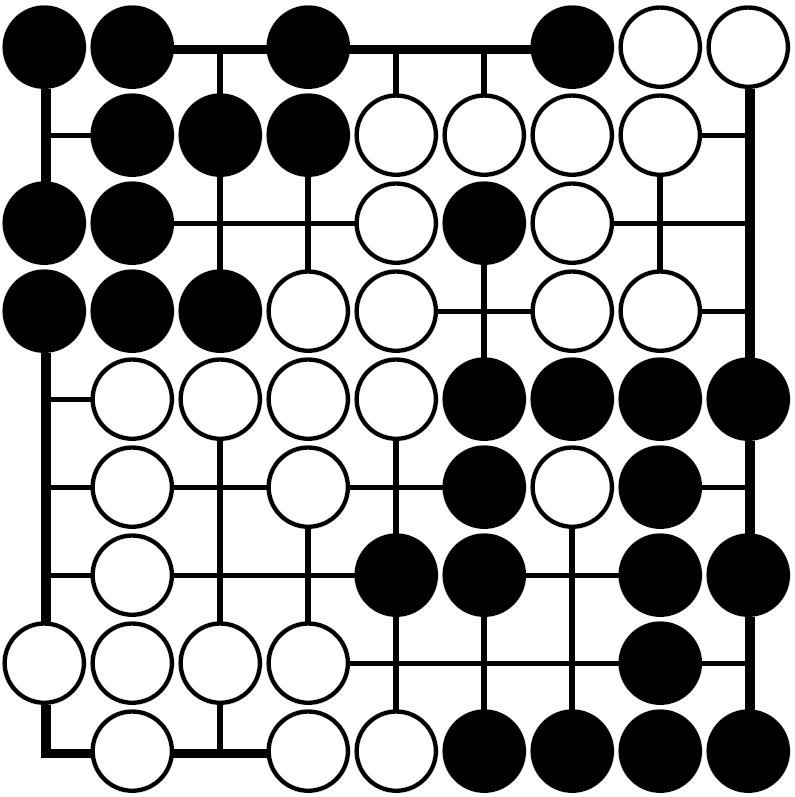
\includegraphics[width=.4\textwidth]{../img/late_endgame_Go_position_suited_for_exact_analysis.png}
    \caption{Late endgame position suited for exact analysis (\cite{Muller1995computer})}
    \label{fig:late-Go-endgame}
  \end{figure}

  Board partition improves when many safe walls are on~the board.
  In the opening and midgame, any partition can be approximate at best.
  In the endgame, the partition gets more precise when the status of~all big groups has been settled, and the outlines of~territories are clear.
  When stones become ``immortal'', significant parts of~the board definitely belong to one of the players.
  The connected components of~the rest of~the board form local games that are independent from each other.

  If each local game is simple enough to~analyze completely (such as in Figure~\ref{fig:late-Go-endgame}), combinatorial game theory can compute an~optimal move for the full board position.
\end{quotation}

\subsection{Playing Computer Go as a~Sum of~Local Games}

This is the general procedure for playing Go as a~sum of~local games used in~(\cite{Muller1995computer}):
\begin{enumerate}
  \item Board partition: find safe blocks, safe territories, and local areas.
  \item Generate local game trees in each area.
  \item Evaluate local terminal positions.
  \item Transform local game trees into mathematical games (and simplify games).
  \item Find an optimal move in the sum game and play it.
\end{enumerate}
\Mueller{} proposes heuristic algorithms for playing the entire game, and exact algorithms for late endgame positions.
Thus, the task of~solving endgames in 1995---at the age of Computer Go's infancy---already played a~vital role.

\subsection{A~Combinatorial Game Theory Framework for Approximate Play of~Sum Games}

\Mueller{} also suggests to replace the ``standard model'' of~computer Go by a~sum game model.
The following benefits and problems of~the sum game model for computer Go are listed in~(\cite{Muller1995computer}):

\medskip

\underline{Benefits}
\begin{itemize}[+]
  \item The model is well suited to the knowledge and style of~\textit{(at that time)} current Go programs:
    they concentrate on local fighting and surrounding territories.
  \item Locality reduces the complexity of~move generation and position evaluation.
    With the emphasis on~evaluation, clever pruning during move generation is not as crucial as in~global search because of~the reduced search space.
  \item Stepwise, directed expansion of~search is supported.
    This provides more time control than the usual iterative deepening.
    It is easy to use opponent's time.
  \item Important Go terms can be expressed or~refined in terms of~the theory, and need not be programmed separately.
  \item The reuse of~local game analysis improves efficiency while playing a~game.
  \item Parallelism emerges naturally on~many levels: local searches are independent, evaluation and operations on mathematical games can be parallelized.
\end{itemize}

\underline{Problems}
\begin{itemize}[-]
  \item Managing incrementally changing sets of~local graphs in place of a single position adds complexity.
  \item Accurate board partition and recognition of~dependencies is crucial.
  \item The usual problems of~selective search appear in complicated local games:
    missing crucial moves leads to wrong evaluation.
  \item Non-constant local games may be overlooked completely, such as insecure ``territories'' which can be destroyed from the inside.
  \item In this model there is no concept of~long-range full board plans.
    This is probably not a~big issue until programs reach amateur Dan or even professional level \textit{(for an~update on the current situation, see Section~\ref{sec:AlphaGo})}.
\end{itemize}

\subsection{A~Sum Game Model for the Entire Game of~Go}

Citing~(\cite{Muller1995computer}), there are several obstacles of~heuristic board partition (in the sum game model).

\begin{enumerate}[(a)]
  \item the impossibility of a~perfect, precise split:
    \begin{quotation}
      When applying a~local game model to the opening or~midgame, the biggest obstacle is the fact that the board cannot be partitioned into independent subgames.
      Few areas are completely surrounded, and surrounding stones are not yet invulnerable.
      We develop heuristics for board partition that split the imperfectly surrounded areas of~the opening and midgame.
    \end{quotation}

  \item the dependencies between the resulting subgames: 
    \begin{quotation}
      An~unavoidable side effect of~heuristic partition are dependencies between the resulting local games.
      Simple strategies for dealing with dependencies are pretending the games are independent, or re-searching a~bigger merged game.
    \end{quotation}
    See Section~\ref{ssec:dependencies-of-subgames} for more details.

  \item the difficulty (or almost infeasibility) of~exhaustive search in still quite large subgames:
    \begin{quotation}
      Even after heuristic partition, areas remain that are too big for an~exhaustive search by a~computer Go program, which must produce a~move in a~few seconds or minutes.
      In such big areas we use selective search.
      Tree growth is controlled by limiting the number of~moves generated, and by stopping the search before reaching a~terminal position.

      There are two levels of~search control:
      for the whole sum game, search time must be distributed between local games.
      For each local game, we must decide which nodes to expand and which expert modules to use for search and evaluation.
      A~post-processing stage handles detected dependencies between games.
    \end{quotation}
\end{enumerate}

Hence, the sum game model makes the best sense during the endgame part.
This general principle is as well applicable in poker:
we wait until the late stage of~the game, when it has greater impact to refine and re-solve the reached endgames.

\subsection{Dependencies Between Local Games}
\label{ssec:dependencies-of-subgames}

(\cite{Muller1995computer}) warns against the dangers of~subgame dependencies:

\begin{quotation}
  Dependencies between games occur when the areas of~local games overlap during area expansion, and when constraints of~one local game are related to~another game.
  The effect of~such dependencies differs widely:
  often it is so small that independence is a~useful approximation.
  In cases when a~move works as a~\emph{double threat} however, dependency analysis is crucial.
\end{quotation}

Strategies for dealing with dependencies are:
\begin{itemize}
  \item Ignore the dependency, treat games as independent
  \item Prove that the dependency does not affect the value of~the sum, or play of~the sum game
  \item Merge mutually dependent local games, then re-search the combined game, possibly using previously generated information on single games
  \item Analyze the interaction between local games, then use a~specialized theory to compute the joint game value
\end{itemize}

\subsection{Local Search and Evaluation in the Endgame}

Here is an overview of treating endgames in~(\cite{Muller1995computer}):
\begin{quotation}
  Following board partition, the algorithm for converting a Go endgame into a combinatorial game consists of generation of local game trees, scoring of local terminal positions, and evaluation of local games as mathematical games.
  Finally, a move in the resulting sum game must be selected, and identified with a move in the Go position.

  Safe territories and dame points are games that can be evaluated statically.
  Other local games are analyzed by local game tree search.
  Terminal positions are evaluated, and the values backed up in the tree, resulting in a mathematical game evaluation of each node.

  The result of search and analysis is a complete description of possible endgame plays that makes perfect play possible.
  We save the results of local analysis in a database of local positions.
  During play, each full board position corresponds one-to- one to a set of local positions, one from each local game.
  Positions and their values are retrieved from the database.

  The value of a full board position is the sum of local position values.
  A sum game evaluation algorithm selects a sufficiently good or optimal move.
  We also consider an algorithm with lower memory requirements, which stores only a subset of the positions of a local game in the database.
  In this case, if play reaches a position not stored in the database, we must re-search the corresponding local game.
\end{quotation}
In greater details, there are several points and aspects worth mentioning:
\begin{enumerate}[(a)]
  \item endgame area
    \begin{quotation}
      An~endgame area consists of~unsettled stones, and of~empty points not yet surrounded by~either color.
      Safe stones, usually of~both colors, surround the area.
      During endgame play, unsettled stones either become safe or are captured.
      Empty points will become occupied, safe territory or dame.
      A~rare case are ``untouchable'' empty points in \emph{seki}.

      \begin{figure}[H]
        \centering
        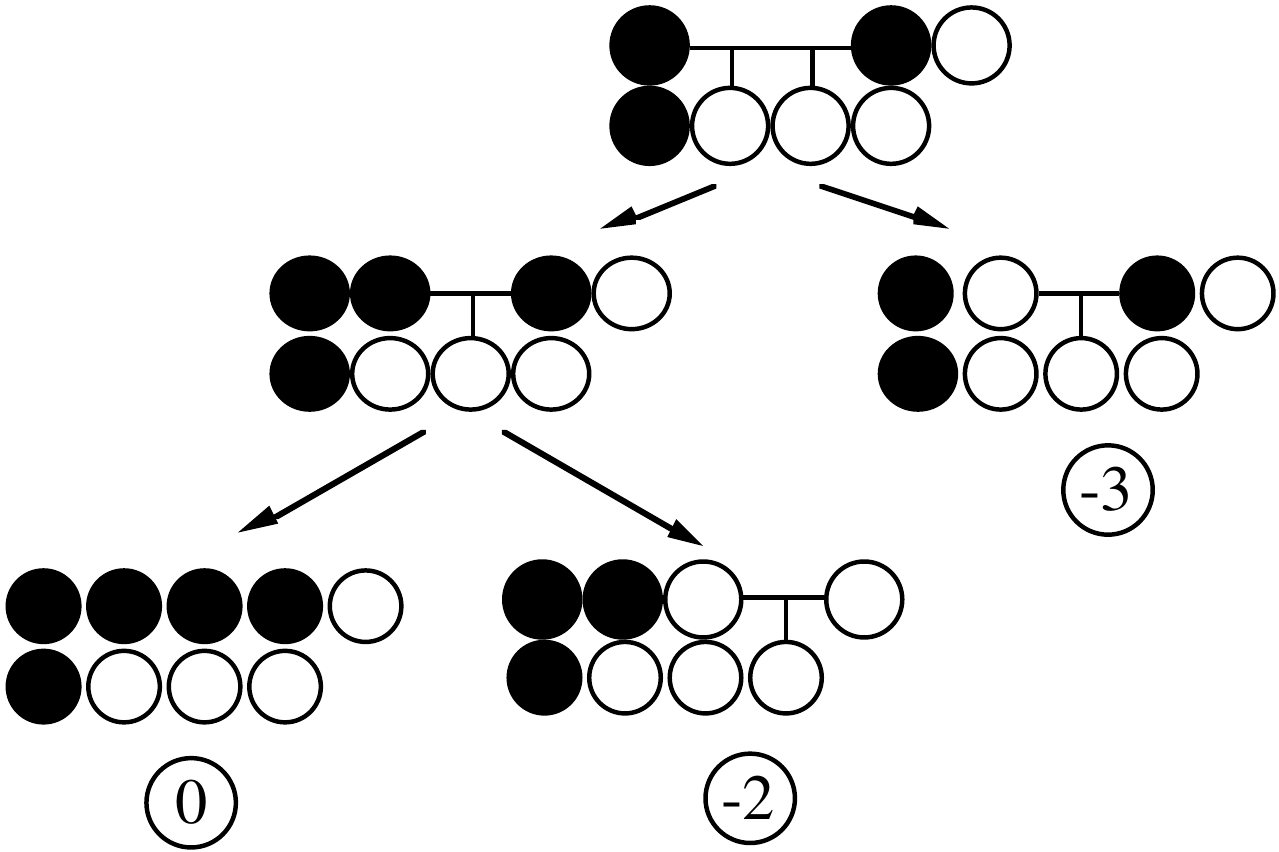
\includegraphics[width=.7\textwidth]{../img/Go_search_tree.png}
        \caption{Local game tree with evaluation of terminal nodes (\cite{Muller1995computer})}
      \end{figure}
    \end{quotation}

  \item move generation
    \begin{quotation}
      We generate all legal moves for both colors, except in a~terminal position or if moves can be pruned.
      Examples of~\emph{pruning rules} are restricting the number of~\emph{dame} moves generated to at most one, and pruning moves dominated by other moves.%
      \footnote{Compare with \emph{policy networks} of~AlphaGo in Section~\ref{sec:AlphaGo}.}
      \emph{Termination rules} decide when a~position can be evaluated statically, without further expanding the tree.%
      \footnote{Compare with \emph{value network} of~AlphaGo in Section~\ref{sec:AlphaGo}.}
    \end{quotation}

  \item terminal positions
    \begin{quotation}
      \noindent
      We recognize the following terminal positions:
      \begin{enumerate}[$\diamondsuit$]
        \item No legal moves
        \item No good move (all points are territory, or dame)
        \item Value of position known from transposition table, pattern, or local position database
      \end{enumerate}
      The first two types of~terminal positions evaluate to a~number, or number-plus-star (odd
      number of~dame).
      If the value of a~position is known from another source, it is terminal in the sense that there is no need to continue search.
      The value itself can be any mathematical game value.
      Non-terminal positions may have a~constant value as well, if the outcome is the same no matter who plays first, but this has to be proven using search.
    \end{quotation}

  \item scoring
    \begin{quotation}
      Scoring assigns a~number, or number plus dame, to a~terminal position.
      In Chinese rules, scoring measures how many stones and empty points belong to either color.
      In Japanese rules, territory and prisoners are counted.
      Both kinds of~scoring are straightforward in the endgame because safe and dead stones, territories and neutral points are known exactly.%
      \footnote{See Subsection~\ref{ssec:rules-Go}.}
    \end{quotation}

  \item exact play on a~subset of~the board
    \begin{quotation}
      When board partition indicates that big areas remain, or search cannot solve all small areas, the user interface offers three options:
      \begin{enumerate}[$\diamondsuit$]
        \item Stop playing
        \item Ignore the unsolvable big areas
        \item Use heuristic play in the big areas
      \end{enumerate}
      Even if an original position has been solved, suicidal opponents can cause problems later:
      they might endanger their ``immortal'' stones, which violates our initial assumptions on board partition and generates new unstable positions where optimal play might be very complicated.
    \end{quotation}

  \item saving results of~local search
    \begin{quotation}
      Positions encountered during local search are stored in \emph{a~database of~local games}.
      An~important question is what to store:
      There is a~tradeoff between recomputation time and required storage.
      For building a~permanent database, it makes sense to store only ``difficult'' moves in the database, and recalculate the rest if needed.
      It is efficient to store which moves are locally good or bad, but omit refutations:
      the trees proving that bad moves are inferior.
      Such a~database is sufficient for playing against a~good opponent.
      Only in the unlikely case of~locally bad opponent play, we must recalculate one subtree to find a~refutation.
      The Table~\ref{tab:db-loc-games} lists some possibilities.
    \end{quotation}
    \begin{table}[!htbp]
      \centering
      \begin{tabular}{ |p{.45\textwidth}|p{.48\textwidth}| } 
        \hline
        \textbf{Type of database} & \textbf{Content} \\
        \hline
        Full                            & All positions encountered during exhaustive search \\
        Color-complete (Black or White) & All positions reachable by non-dominated moves of~color and arbitrary opponent moves (pruned bad moves of~color) \\
        Optimal                         & At least one position corresponding to each non-dominated option of each reachable position, guarantees optimal play from each position in~database \\
        Ko-complete (Ko-optimal)        & Complete (optimal) + possible Ko threats and answers \\
        Sufficiently good               & Guarantees optimal score from a~starting position, might fail to exploit some opponent mistakes \\
        \hline
      \end{tabular}
      \caption{Possible database variants of~local games}
      \label{tab:db-loc-games}
    \end{table}

  \item pruning game trees 
    \begin{quotation}
      The evaluation of~nodes leads to pruning the game tree:
      moves to dominated options are marked as locally bad moves.
      With the usual domination test for $\geq$, all but the first of~several equally good moves are pruned.
      A~test for $>$ keeps the full set of~equally good moves.
    \end{quotation}

  \item mapping a~move in the abstract game to a~Go move
    \begin{quotation}
      As a~last step, we must find a~Go move corresponding to the selected option in the abstract game.
      We select the first move with sufficient \emph{incentive}.
    \end{quotation}
\end{enumerate}

\clearpage

\subsection{Speeding up Local Search}

(\cite{Muller1995computer}) considers various improvements to computational efficiency:
\begin{quotation}
  Ignoring illegal moves and captures, the number of possible plays in an $n$ point area is approximately $2n$ ($n$ for each player), and play generates a $n-1$ point area.
  A~rough estimate for the size of~the game tree is therefore $2n\cdot2(n-1)\cdot \ldots \cdot2 = 2^n n!$

  Due to this combinatorial explosion, even fairly small endgames become prohibitively expensive to compute using this approach.
  In the following, we look at a~number of~techniques for reducing the size of the search tree.
\end{quotation}

\begin{enumerate}[(a)]
  \item transposition table (see also Table~\ref{tab:reduction-transp-tab})
    \begin{quotation}
      A~transposition table detects identical board positions, reducing the size of~the search space from $\approx 2^n n!$ to $3^n$ states.

      \begin{table}[!htbp]
        \centering
        \begin{tabular}{ |rrr| }
          \hline
          \textbf{$n$} & \textbf{$2^nn!$} & \textbf{$3^n$} \\
          \hline
          1	&	2	&	3 \\ 
          2	&	8	&	9 \\ 
          3	&	48	&	27 \\ 
          4	&	384	&	81 \\ 
          5	&	3840	&	243 \\ 
          6	&	46080	&	729 \\ 
          7	&	645120	&	2187 \\ 
          8	&	10321920	&	6561 \\ 
          9	&	185794560	&	19683 \\ 
          10	&	3715891200	&	59049 \\ 
          \hline
        \end{tabular}
        \caption{Reduction of search space by transposition table}
        \label{tab:reduction-transp-tab}
      \end{table}
    \end{quotation}

  \item pruning moves
    \begin{quotation}
      The width of~the search tree can be further reduced by pruning moves.
      In contrast to selective search, we may only eliminate moves that are provably worse-or-equal than others.
      If a~move achieves all points of~the local area, or if any other move would give the opponent an~answer which achieves the maximum score, the move is optimal, and we can prune all other moves.
    \end{quotation}
\end{enumerate}

\subsection{Using Combinatorial Game Theory to Solve Late Endgames by Computer}

These are some objectives that can be accomplished by the approach of~(\cite{Muller1995computer}):
\begin{itemize}
  \item Perfect computer play in late endgame
  \item Find the game-theoretic value of a position long before the end
  \item Evaluate the opponent’s endgame moves
  \item Find moves that are good enough even with a reduced local game database
\end{itemize}
On the other hand, the work also remarks that strict analysis of~endgames is not possible with this method if one of the following limits is reached:
\begin{itemize}
  \item \textbf{Partition:}
    too few blocks can be proven safe independent of~endgame play.
    Therefore some areas become too big for complete search.
  \item \textbf{Summation:}
    no move with dominating incentive exists, and both summing and partial search take too long.
  \item \textbf{Ko:}
    Standard combinatorial game theory exploits the independence of~local games.
    In the case of~Ko, the independence is broken (a~locally bad move may be globally best if it serves as a~Ko threat).
    Generalizations of~the theory to handle Kos are a topic of [at that time] current research.
  \item \textbf{Added complexity in ‘obvious’ situations:}
    In cases where the focus of~play is obvious (i.e. only one local situation is relevant), combinatorial game theory introduces additional complexity by investigating moves for both players in this and each other position.
\end{itemize}

\subsection{Time and Memory Management}

One reason why endgames are exhaustively studied is due to their computational benefits.
As the game progresses, more exact analysis can be done, and thus, time and memory resources may be better utilized.
In particular, (\cite{Muller1995computer}) uses following ``adaptive'' resource adjustments:

\begin{enumerate}[(a)]
  \item memory management of objects and local trees
    \begin{quotation}
      In a~program with limited memory, we need to decide which local game nodes and other calculated results to keep, and which to dispose during the course of play.
      Which items are obsolete, and which can probably be reused later?
      Only heuristic rules for memory management are possible, because the future actions of~the user are unpredictable.

      During the course of a~game there is a~gradual shift of~relevance.
      Starting a~new game leads to radical change, just about all computed results are useless in the new game.
      Some flexibility for users undoing moves should be provided.

      As a~solution we define a~\emph{forced substate}, a subset of all points on the current board.
      The substate consists mainly of~safe-looking stones.
      We delete all objects that do not match the forced substate.
      For supporting undo’s, we exclude all points affected by the last two moves from the points of~the forced substate.
      Some items are exempt from automatic disposal:
      user inputs, and objects explicitly calculated on a~user’s demand.
    \end{quotation}

    \parbox{.9\textwidth}{
    \item time control for tournament play
      \begin{quotation}
        Time control determines how much time to use for each subgame, for tactics, and for
        Life\&Death problems. [$\dots$]
        The same algorithm with smaller time slices could be used for computing in opponents time.
        A~fast mode is used in time trouble:
        only minimal time is used for subproblems such as tactics calculations and Life\&Death.
      \end{quotation}
    }

\end{enumerate}

\subsection{Pattern Learning}

Pattern recognition is one of~the key components of~AlphaGo.
Arguably, the program's success might be partially attributed to learning Go patterns from human expert plays (see Section~\ref{sec:AlphaGo}).
For comparison, (\cite{Muller1995computer}) suggested pattern matching as a~promising mean for improvement:

\begin{quotation}
  Research on pattern learning in computer Go has unfortunately been restricted to \emph{ab-initio} learning of~the most basic patterns from zero knowledge.
  Interactive or automatic tuning and expansion of a~state-of-the-art pattern base is another fascinating research topic.
\end{quotation}

\subsection{Contributions of~Combinatorial Game Theory to Go Endgames}

The doctoral thesis (\cite{Muller1995computer}) highlights following contributions to general computer science:
\begin{itemize}
  \item Scientists are fascinated by problems which can be stated simply, yet are hard to solve.
    Computer Go is a~prime example.
    We have brought the divide-and-conquer approach, a~fundamental paradigm of~computer science, to bear on computer Go.

  \item The application of a~sophisticated mathematical theory to computer Go provides an~example of~algorithms for a~nontrivial decomposition of a~complex problem.
\end{itemize}
Another contributions are the ones aiding computer Go endgames specifically:
\begin{itemize}
  \item We have implemented a~\emph{late endgame player}, a~niche where program play surpasses human play in both speed and exactness.
    We did this by applying concepts from combinatorial game theory to Go.
    The program plays a~wide variety of`late endgame positions perfectly.

  \item We have developed algorithms for board partition and dependency analysis.
    The central idea of~board partition has been used both in a~program following a~traditional model, and in a~program based on the sum game approach.
\end{itemize}
Hence, the work employs a~technique of~applying an~elaborate mathematical theory (of~combinatorial game theory) to deal with the endgame phase.
In particular, CGT is used to ``connect'' individual relevant subgames, which may be solved independently.

As we will see later, the situation in the case of~Poker is slightly more delicate:
the imperfect-information property prevents us from using an~immediate divide-and-conquer approach.
Instead, we will \emph{augment} the information by saturating it with additional game states (see Section~\todo).

\note{
  \label{note:CGTvsAlphaGo}
  It is also interesting to compare the method of~(\cite{Muller1995computer}) with the modern approach of~\emph{AlphaGo}:
  the ad-hoc Go-specific knowledge is replaced with general-learning neural networks and the probabilistic \emph{Monte Carlo Tree Search} algorithm.
  Such a~combination has the capability to surpass professional human players at the highest ranks.
  On top of that, this solution can be adapted to other games without substantial modifications.
  As long as there is an~abundance of~available data, the system can always be trained with no need to imbue it with any game-specific knowledge.
  See Section~\ref{sec:AlphaGo} for more details.
}

\clearpage

\section{Go Endgames Using Artificial Intelligence}
\label{sec:AlphaGo}

The game of Go has long been viewed as the most challenging of classic games for artificial intelligence owing to its enormous search space and the difficulty of evaluating board positions and moves.
A~new approach to computer Go introduces \emph{value networks} to evaluate board positions and \emph{policy networks} to select moves.
These deep neural networks are trained by a novel combination of supervised learning from human expert games, and reinforcement learning from games of self-play.

Furthermore, a~new search algorithm is introduced: it combines Monte Carlo simulation with value and policy networks.
Using this search algorithm, the computer program AlphaGo developed by~Google DeepMind achieved a~99.8~\% winning rate against other Go programs.~(\cite{Silver2016mastering})

\todo
